\documentclass[a4paper,11pt,noarxiv]{quantumarticle}
% Supplemental Material for "Lattice refinement followed by the rodeo
% algorithm: a gate-level benchmark of eigenstate-preparation routes on the
% Hubbard chain" (paper III).  Cross-references to the main text resolve
% through xr against eigenq_hubbard.aux (compile the main text first).
% Every number traces to notebooks/ResolutionRefHubbard.ipynb.
\usepackage[utf8]{inputenc}
\usepackage[T1]{fontenc}
\usepackage{amsmath,amssymb}
\usepackage{physics}
\usepackage{graphicx}
\usepackage{booktabs}
\usepackage{xcolor}
\usepackage{hyperref}
\usepackage{xr}
\externaldocument{eigenq_hubbard}
\newcommand{\todo}[1]{\textcolor{red}{[#1]}}
\newcommand{\Hlow}{H_{\mathrm{low}}}
\newcommand{\Hhigh}{H_{\mathrm{high}}}
\newcommand{\Eobj}{E_{\mathrm{obj}}}
\newcommand{\Deff}{\Delta_{\mathrm{eff}}}
\renewcommand{\thesection}{S\arabic{section}}
\renewcommand{\thefigure}{S\arabic{figure}}
\renewcommand{\thetable}{S\arabic{table}}
\renewcommand{\theequation}{S\arabic{equation}}

\begin{document}
\title{Supplemental Material for ``Lattice refinement followed by the rodeo
algorithm: a gate-level benchmark of eigenstate-preparation routes on the
Hubbard chain''}
\author{Scott Bogner}
\affiliation{Facility for Rare Isotope Beams and Department of Physics and Astronomy, Michigan State University, East Lansing, MI 48824, USA}
\author{Cecilie Glittum}
\affiliation{Department of Physics, University of Oslo, N-0316 Oslo, Norway}
\author{Heiko Hergert}
\affiliation{Facility for Rare Isotope Beams and Department of Physics and Astronomy, Michigan State University, East Lansing, MI 48824, USA}
\author{Morten Hjorth-Jensen}
\email{mhjensen@uio.no}
\affiliation{Department of Physics, University of Oslo, N-0316 Oslo, Norway}
\author{Gunnar Lange}
\affiliation{Department of Physics, University of Oslo, N-0316 Oslo, Norway}
\author{Ryan LaRose}
\affiliation{Department of Computational Mathematics, Science and Engineering and Facility for Rare Isotope Beams, Michigan State University, East Lansing, MI 48824, USA}
\author{Dean Lee}
\affiliation{Facility for Rare Isotope Beams and Department of Physics and Astronomy, Michigan State University, East Lansing, MI 48824, USA}
\author{Francesco Pietro Massel}
\affiliation{Department of Science and Industry Systems, University of South-Eastern Norway, N-3616 Kongsberg, Norway}
\affiliation{Department of Physics, University of Oslo, N-0316 Oslo, Norway}
\author{Jean Paul Sadia}
\affiliation{Department of Computational Mathematics, Science, and Engineering, Michigan State University, East Lansing, MI 48823, USA}
\affiliation{Center for Quantum Computing, Science, and Engineering, Michigan State University, East Lansing, MI 48823, USA}
\maketitle

This Supplemental Material collects the verification material behind the
main text: the sufficient adiabatic time and the response norm of the path
(Sec.~\ref{sm:bound}), the dimer-seeded hierarchy and the composition of
steps (Sec.~\ref{sm:dimer}), the plaquette spectra (Sec.~\ref{sm:2d}), the
variational tables (Sec.~\ref{sm:uccsd}), the Trotterized refinement at
eight sites (Sec.~\ref{sm:trotter}), the exact-ensemble filter
(Sec.~\ref{sm:filter}), the ingredients and validation of the
thirty-two-qubit study (Sec.~\ref{sm:large}), and the operating-point tables
(Sec.~\ref{sm:ops}).  Equation, section, table and figure numbers without
the prefix S refer to the main text; all numbers are outputs of the
notebook \texttt{notebooks/ResolutionRefHubbard.ipynb}.

% ===========================================================================
\section{The sufficient adiabatic time and the response norm of the path}
\label{sm:bound}
% ===========================================================================
Table~\ref{tab:bound} evaluates the sufficient adiabatic time of Jansen,
Ruskai and Seiler~\cite{Jansen2007} in the form used in paper I,
$T_b=\epsilon^{-1/2}\int_0^1[\|\ddot H\|/\Delta^2+7\|\dot H\|^2/\Delta^3]\,ds$
with $\|B-A\|$ the spectral norm of $\Hhigh-P\Hlow P^\dagger$ in the sector,
once with the sector gap and once with the gap in the symmetry sector of the
tracked state (Fig.~\ref{fig:gaps}), against the empirical $T^*$.  The
symmetry-resolved bound is smaller by a factor $5$ to $17$ but remains three
to five orders of magnitude above $T^*=10/t$, as the pairing bound did
(there $3\times10^2$); the larger ratio here reflects $\|B-A\|=11$--$20$,
set by the shift $\mu$ and the width of the Hubbard spectrum.  The bound
guarantees a worst-case operator-norm error for every initial state in the
branch, $T^*$ records one overlap for one initial state, so the ratio
measures the slack of the criterion, not an error in either.

\begin{table*}[t]
  \caption{Sufficient adiabatic time $T_b$ (infidelity $\epsilon=10^{-2}$)
  along Path~A ($\mu_{\rm buf}=2t$) for the chain $4\to8$, evaluated with the
  sector gap and with the gap in the symmetry sector of the tracked state,
  against the empirical $T^*$ ($1-p<10^{-3}$).  Times in units of $1/t$.}
  \label{tab:bound}
  \centering\scriptsize
  \begin{tabular}{ccccccc}
  \toprule
  $U/t$ & $\min\Delta$ & $\min\Deff$ & $\|B-A\|$ & $T_b(\Delta)$ & $T_b(\Deff)$ & $T^*$\\
  \midrule
  0 & 0.532 & 0.879 & 11.1 & $5.7\times10^{4}$ & $1.2\times10^{4}$ & 10\\
  2 & 0.319 & 0.780 & 11.8 & $2.5\times10^{5}$ & $2.0\times10^{4}$ & 10\\
  4 & 0.223 & 0.588 & 13.9 & $1.0\times10^{6}$ & $6.4\times10^{4}$ & 10\\
  8 & 0.137 & 0.366 & 20.0 & $1.0\times10^{7}$ & $5.8\times10^{5}$ & 10\\
  \bottomrule
  \end{tabular}
\end{table*}

The first-order response norm of the path,
$\chi_u(s)=\sum_{n>0}|\langle n(s)|\partial_uH|0(s)\rangle|^2/[E_n(s)-E_0(s)]^2$
with $u=\sin^2(\pi s/2)$ and $\partial_uH=(\Hhigh-\mu)-P(\Hlow-\mu)P^\dagger$,
is the quantity whose integral along the path sets the adiabatic leakage at
leading order; for the pairing model paper I obtained it in closed form at
the start of the path, $\chi_u(0)=g^2/\mu_{\rm buf}^2$.
Figure~\ref{fig:ramp} (left) follows it along Path~A for the chain $4\to8$:
$\chi_u(0)=0.375$, $0.527$, $0.715$ and $0.874$ for $U/t=0,2,4,8$, the
maximum sits at the initial endpoint for every coupling, and the norm falls
by a factor two to four along the path (at $U=8t$ it rises again toward
$s=1$, to $0.45$, as $\Deff$ shrinks).  The shift fixes the initial value as
it did for the pairing model, and the growth of $\chi_u(0)$ with $U$ is
modest, in line with the flat $T^*$.  The right panel compares, with exact
slices, the ordinary adiabatic ramp from the free-fermion determinant with
the two refinement paths at $U=4t$: the ramp reaches $p=0.96878$,
$0.99686$, $0.99960$ and $0.99989$ at $T=4,8,12,16$ (and $0.99999$ at
$24/t$).

\begin{figure*}[t]
  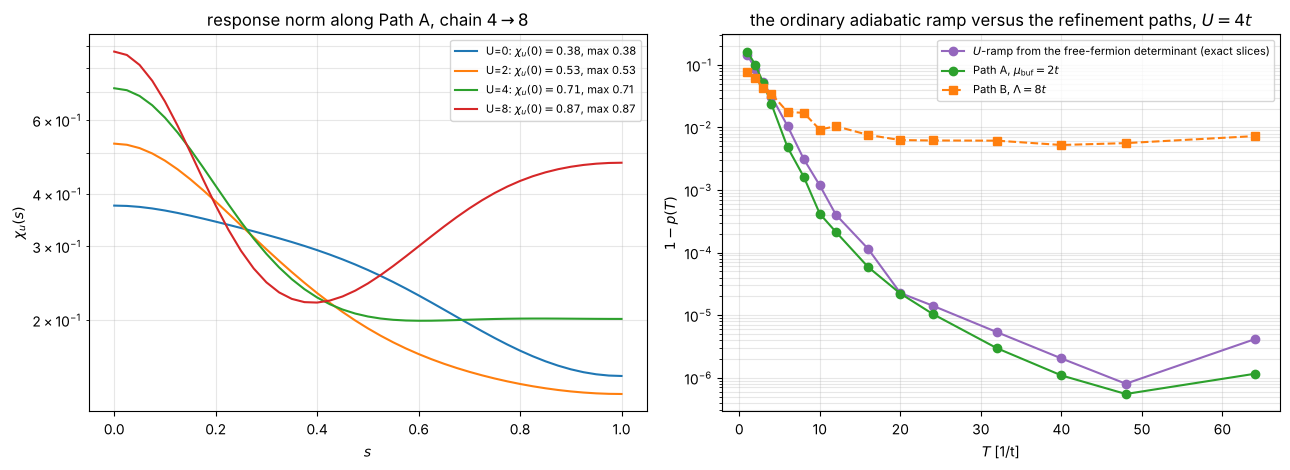
\includegraphics[width=\textwidth]{figs/fig9.png}
  \caption{Left: the first-order response norm $\chi_u(s)$ along Path~A
  ($\mu_{\rm buf}=2t$) for the chain $4\to8$ at $U/t=0,2,4,8$; the maximum
  sits at the initial endpoint for every coupling.  Right: $1-p(T)$ with
  exact slices for the ordinary adiabatic ramp from the free-fermion
  determinant, for Path~A and for Path~B ($\Lambda=8t$) at $U=4t$.}
  \label{fig:ramp}
\end{figure*}

% ===========================================================================
\section{The dimer-seeded hierarchy and the composition of steps}
\label{sm:dimer}
% ===========================================================================
Table~\ref{tab:dimer} shows the first step of the one-dimensional
hierarchy, from the filled dimer ($N_\uparrow=N_\downarrow=2$, one state,
$E_{\rm low}=U-4t$) to the four-site chain: the doubly-occupied seed is a
worse start as $U$ grows, $p_0=0.80$ at $U=0$ down to $0.48$ at $U=8t$, but
the effective gap is large ($\Deff=2.2t$--$0.8t$) and $p>0.9997$ is reached
by $T=16/t$ at every $U$.  Figure~\ref{fig:composed} composes the steps
(Sec.~\ref{sec:dimer}): with the refined four-site state as the input of the
$4\to8$ step and the shift referenced to its variational energy
$\expval{\Hlow}{\psi}$, the chain $2\to4\to8$ at $U=4t$ with $T=16/t$ per
step reaches $p=0.99988$ against $0.99994$ from the exact coarse input; with
$T=8/t$ in the first step the second saturates at $p=0.9979$, the overlap
of its input.  The single-shot refinement $2\to8$ with blocks of four fine
sites starts from $p_0=0.579$ and reaches $p=0.9966$ at $T=16/t$ and
$0.99988$ only at $T=32/t$.

\begin{table*}[t]
  \caption{The first step of the one-dimensional hierarchy: the filled dimer
  ($N_\uparrow=N_\downarrow=2$, one state) refined to the four-site open chain
  (36 states), Path~A with $\mu_{\rm buf}=2t$.}
  \label{tab:dimer}
  \centering\scriptsize
  \begin{tabular}{cccccccc}
  \toprule
  $U/t$ & $E_{\rm low}$ & $E_{\rm high}$ & $p_0$ & $\Delta$ & $\Deff$ & $p(8)$ & $p(16)$\\
  \midrule
  0 & $-4$ & $-4.4721$ & 0.805 & 1.236 & 2.236 & 0.9999 & 1.0000\\
  2 & $-2$ & $-2.8759$ & 0.754 & 0.789 & 1.851 & 0.9995 & 1.0000\\
  4 & $\phantom{-}0$ & $-1.9531$ & 0.645 & 0.540 & 1.358 & 0.9979 & 0.9999\\
  8 & $\phantom{-}4$ & $-1.1172$ & 0.480 & 0.311 & 0.805 & 0.9787 & 0.9997\\
  \bottomrule
  \end{tabular}
\end{table*}

\begin{figure*}[t]
  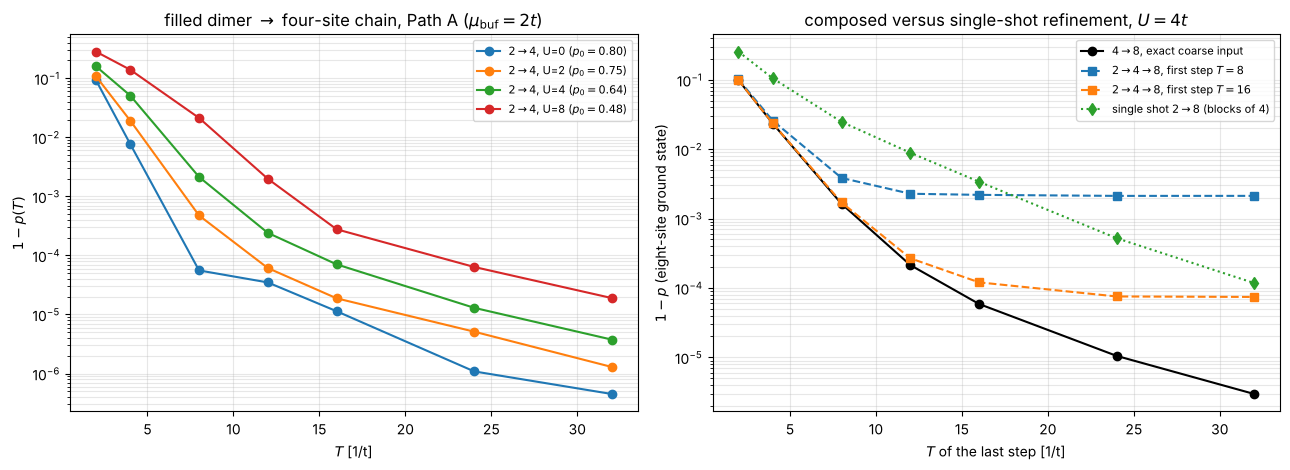
\includegraphics[width=\textwidth]{figs/fig4.png}
  \caption{Left: $1-p(T)$ for the dimer step $2\to4$ at $U/t=0,2,4,8$.
  Right, $U=4t$: the step $4\to8$ from the exact coarse ground state
  (circles), the composed chain $2\to4\to8$ with the refined four-site state
  as input after a first step of $T=8/t$ or $16/t$ (squares), and the
  single-shot refinement $2\to8$ with blocks of four fine sites (diamonds),
  all versus the time of the last step.}
  \label{fig:composed}
\end{figure*}

The step $8\to16$ at $(2,2)$, $U=4t$ ($784\to14\,400$ states) starts from
$p_0=0.869$ with $E_{\rm low}=-6.817213$ and $E_{\rm high}=-7.209813$.
Among the forty lowest eigenstates of the fine sector the first to carry
weight lies at $\Deff=0.138t$ (weight $10^{-4}$), the next at $0.415t$ and
$0.505t$ (the latter with weight $10^{-2}$), while the eight other states
below $0.4t$, including the one that defines the sector gap ($0.051t$),
carry none.  With $\mu_{\rm buf}=2t$ the overlap reaches $0.9924$, $0.99931$
and $0.99995$ at $T=8,16,32$; composing three steps from the filled dimer,
$2\to4\to8\to16$ with $T=16/t$ each and the refined state as the input of
every step, gives $p=0.99923$.

% ===========================================================================
\section{The plaquette}
\label{sm:2d}
% ===========================================================================
Table~\ref{tab:2d} collects the plaquette refinements of
Sec.~\ref{sec:2d}.  At $(2,2)$ the fine ground state has weight $0$ on the
prolonged coarse ground state ($B_1$ singlet), $0.647$ on the prolonged
$A_2$ triplet, and $0.007$ on all other coarse states together ($U=4t$);
the lowest state of the $(A_2,S=1)$ sector that carries weight lies $1.77t$
above the ground state (among the thirty lowest eigenstates).  The $U=0$
point is degenerate in both models and its labels are not meaningful.

\begin{table*}[t]
  \caption{Plaquette refinement $2\times2\to4\times4$ on the open square
  lattice, Path~A with $\mu_{\rm buf}=2t$.  At $(2,2)$ the coarse ground
  state is a $B_1$ singlet with zero overlap on the $A_2$ triplet ground
  state of the fine lattice; the last row refines the lowest coarse
  $(A_2,S=1)$ state, and $\Deff$ is taken among the thirty lowest fine
  eigenstates.}
  \label{tab:2d}
  \centering\scriptsize
  \begin{tabular}{cccccccccc}
  \toprule
  $(N_\uparrow,N_\downarrow)$ & $U/t$ & dims & $E_{\rm low}$ & $E_{\rm high}$ & $(\Gamma,S)$ coarse / fine & $p_0$ & $\Delta$ & $\Deff$ & $p(16)$\\
  \midrule
  (1,1) & 0 & $16\to256$ & $-6.0000$ & $-6.4721$ & $A_1$ / $A_1$ & 0.805 & 1.000 & 2.236 & 0.99999\\
  (1,1) & 4 & $16\to256$ & $-5.8136$ & $-6.2638$ & $A_1$ / $A_1$ & 0.840 & 0.792 & 2.096 & 0.99999\\
  (1,1) & 8 & $16\to256$ & $-5.7093$ & $-6.1833$ & $A_1$ / $A_1$ & 0.845 & 0.711 & 2.129 & 0.99998\\
  (2,2) & 4 & $36\to14\,400$ & $-9.4142$ & $-10.4197$ & $(B_1,0)$ / $(A_2,1)$ & 0 & 0.090 & --- & $3\times10^{-27}$\\
  (2,2) & 4 & $36\to14\,400$ & $-9.3429$ & $-10.4197$ & $(A_2,1)$ / $(A_2,1)$ & 0.647 & 0.090 & 1.771 & 0.99997\\
  \bottomrule
  \end{tabular}
\end{table*}

% ===========================================================================
\section{The variational inputs}
\label{sm:uccsd}
% ===========================================================================
Table~\ref{tab:uccsd} collects the single-layer UCCSD results.  On the
coarse chain the 26-parameter ansatz is exact at $U=0$ and reaches
infidelities $1.8\times10^{-4}$, $3.3\times10^{-3}$ and $1.7\times10^{-2}$
at $U/t=2,4,8$ from a free-fermion reference that is very poor at strong
coupling ($E_{\rm HF}-E_{\rm FCI}=2.3t$ at $U=8t$); on the fine chain the
198-parameter ansatz does slightly better, $4.7\times10^{-4}$,
$3.1\times10^{-3}$, $1.2\times10^{-2}$, at $3.1\times10^4$ CNOTs against
$1.7\times10^3$.  Used as the coarse solver, the UCCSD state is prolonged
with essentially the same $p_0$ as the exact coarse state but the
refinement then saturates at $p=0.99669$ ($U=4t$) and $0.98234$ ($U=8t$)
instead of $0.9999$.  At $U=4t$, $72$ of the $198$ fine-chain amplitudes
exceed $10^{-2}$ and $98$ exceed $10^{-3}$; keeping those $98$ ($12$
singles, $86$ doubles) and re-optimizing from the converged values gives
$E=-5.618755$ and $1-F=3.145\times10^{-3}$ against $-5.618758$ and
$3.143\times10^{-3}$ for the full pool, at $15\,120$ against $30\,864$
CNOTs.  At sixteen sites the single-layer ansatz has $1\,022$ parameters
($E=-7.197325$ against $E_0=-7.209813$, $1-F=6.98\times10^{-3}$,
$335\,360$ CNOTs) and its pruned version $255$ parameters
($7.00\times10^{-3}$, $87\,776$ CNOTs).

\begin{table*}[t]
  \caption{Sector-level UCCSD on the Galerkin coarse chain ($L=4$,
  Eq.~\eqref{eq:gal1d}) and on the fine chain ($L=8$) at $(2,2)$:
  reference, variational and exact energies, infidelity with the exact
  ground state, number of parameters and CNOT count of the preparation
  (Givens network plus excitation blocks).  The last columns give the
  overlap of the prolonged UCCSD coarse state and its Path-A refinement at
  $T=16/t$.}
  \label{tab:uccsd}
  \centering\scriptsize
  \setlength{\tabcolsep}{3pt}
  \begin{tabular}{c|cccc|cccc|cc}
  \toprule
  & \multicolumn{4}{c|}{coarse $L=4$ (26 parameters, 1720 CNOTs)} & \multicolumn{4}{c|}{fine $L=8$ (198 parameters, 30864 CNOTs)} & \multicolumn{2}{c}{UCCSD coarse $\to$ refined}\\
  $U/t$ & $E_{\rm HF}$ & $E_{\rm UCCSD}$ & $E_{\rm FCI}$ & $1-F$ & $E_{\rm HF}$ & $E_{\rm UCCSD}$ & $E_{\rm FCI}$ & $1-F$ & $p_0$ & $p(16)$\\
  \midrule
  0 & $-6.23607$ & $-6.23607$ & $-6.23607$ & $<10^{-15}$ & $-6.82295$ & $-6.82295$ & $-6.82295$ & $<10^{-14}$ & 0.77733 & 0.99997\\
  2 & $-5.23607$ & $-5.43744$ & $-5.43797$ & $1.8\times10^{-4}$ & $-5.71184$ & $-6.02962$ & $-6.03209$ & $4.7\times10^{-4}$ & 0.81405 & 0.99977\\
  4 & $-4.23607$ & $-4.96957$ & $-4.97657$ & $3.3\times10^{-3}$ & $-4.60073$ & $-5.61876$ & $-5.63443$ & $3.1\times10^{-3}$ & 0.79991 & 0.99669\\
  8 & $-2.23607$ & $-4.51765$ & $-4.55859$ & $1.7\times10^{-2}$ & $-2.37850$ & $-5.22167$ & $-5.27797$ & $1.2\times10^{-2}$ & 0.75667 & 0.98234\\
  \bottomrule
  \end{tabular}
\end{table*}

ADAPT-VQE (Sec.~\ref{sec:uccsd}) is run with gradient tolerance $10^{-6}$
and at most $200$ operators, every amplitude re-optimized by L-BFGS
warm-started from the previous iteration, with the exact ground state used
only to record the infidelity.  At eight sites ($U=4t$, pool of $198$) the
infidelity falls below $10^{-2}$, $3\times10^{-3}$, $10^{-3}$ and
$3\times10^{-4}$ after $66$, $101$, $149$ and $194$ operators ($11\,712$,
$15\,528$, $22\,816$ and $30\,000$ CNOTs including the Givens network;
$2.77\times10^{-4}$ after $200$); at sixteen sites (pool of $1\,022$) it
falls below $10^{-2}$ after $187$ operators ($68\,008$ CNOTs) and reaches
$9.45\times10^{-3}$ after $200$.  The CNOT count of a prefix is that of
its operators as compiled in Sec.~\ref{sec:circuits}.  The eight-site
state at $149$ operators, fed to the Trotterized filter of
Sec.~\ref{sec:budget} with its forty time sets, gives
$1-\mathcal F_M=9.8\times10^{-4}$, $5.1\times10^{-4}$,
$2.8\times10^{-4}$, $1.7\times10^{-4}$, $1.2\times10^{-4}$,
$8.6\times10^{-5}$ and $7.3\times10^{-5}$ for $M=0$--$6$ at
$2.3\times10^4$, $4.5\times10^4$, $6.9\times10^4$, $9.5\times10^4$,
$1.2\times10^5$, $1.5\times10^5$ and $1.7\times10^5$ CNOTs per accepted
preparation.

% ===========================================================================
\section{Trotterized refinement at eight sites}
\label{sm:trotter}
% ===========================================================================
Figure~\ref{fig:trotter} replaces the exact slice propagation at $T=16/t$,
$U=4t$ by first- and second-order product formulas over the groups
$[P(\Hlow-\mu)P^\dagger,\,K_{\rm even},\,K_{\rm odd},\,D-\mu]$ for Path~A
and $[(1+\Lambda\cos^2)K_{\rm even},\,K_{\rm odd},\,D]$ for Path~B.  The
second-order formula reproduces the exact-slice overlap to within $10^{-3}$
with $n_s=128$ steps for Path~A ($p=0.99983$), $256$ for Path~B with
$\Lambda=8t$ ($0.99213$) and $512$ for $\Lambda=16t$ ($0.99342$);
first-order formulas do not reach it within $10^{-3}$ even at $512$ steps.
The counted circuit of Path~A does not exponentiate the embedded coarse
term as one block: on a device it is the coarse Hubbard step, i.e.\ the
three conditioned coarse groups $P(D_c-\mu)P^\dagger$,
$PK^c_{\rm even}P^\dagger$ and $PK^c_{\rm odd}P^\dagger$, which do not
commute.  Repeating the second-order refinement with the coarse term split
accordingly (six groups in all) gives $p=0.997299$, $0.999818$, $0.999941$
and $0.999943$ at $n_s=64$, $128$, $256$ and $512$, against $0.997456$,
$0.999831$, $0.999941$ and $0.999943$ with the coarse term as one block;
the step count $n_s=128$ and the cost of Path~A are unchanged, and the
split-group state is the one used in Table~\ref{tab:budget}.  The ramp's
product-formula version reproduces its exact-slice overlap with $64$
second-order steps at $T=8/t$ ($0.996891$ against $0.996861$) and gives
$0.999659$ (exact $0.999885$) with $128$ steps at $T=16/t$.

The embedded coarse term of Path~A at eight sites is the coarse Hubbard
step on the bonding register --- $24$ rotations, $32$ CNOTs unconditioned
--- with every rotation conditioned on the eight antibonding qubits being
empty.  With the Gray-code phase-polynomial convention of paper I (exact for
few controls but growing as $2^{c+1}$) this is $1.2\times10^4$ CNOTs per
application; with a clean-ancilla ladder of relative-phase Toffolis
($6(c-1)+2$ extra CNOTs per rotation) it is $1\,088$, the figure used
throughout.  In the block Jordan--Wigner ordering the $Z_jZ_{j+L_f}$ terms
are the only non-local ones; the site-major ordering, which makes them
adjacent at the price of weight-three hopping strings, is the alternative
to be compared on a linear-connectivity device.

\begin{figure}[t]
  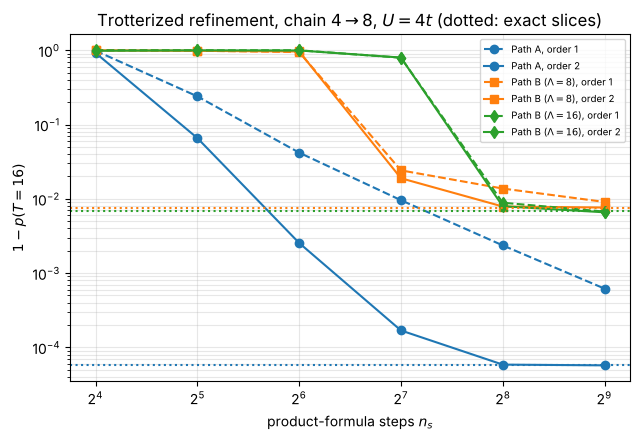
\includegraphics[width=\linewidth]{figs/fig7.png}
  \caption{Trotterized refinement of the chain $4\to8$ at $U=4t$, $T=16/t$:
  $1-p$ versus the number of product-formula steps for Path~A and Path~B
  ($\Lambda=8t$, $16t$), first (dashed) and second order (solid); dotted
  lines are the exact-slice values.}
  \label{fig:trotter}
\end{figure}

% ===========================================================================
\section{The exact-ensemble filter}
\label{sm:filter}
% ===========================================================================
Figure~\ref{fig:rodeo} shows the exact ensemble infidelity,
Eq.~\eqref{eq:fid}, with $\sigma=5/\Deff$ for the inputs of
Sec.~\ref{sec:res-rodeo}.  Applied to the Path-B state at its ceiling
($\Lambda=16t$, $T=32/t$, $1-p\simeq2\times10^{-3}$) the filter reaches
$2$--$4\times10^{-5}$ after six cycles.  The exact-ensemble values lie below
the sampled, Trotterized ones of Table~\ref{tab:budget} once the latter
approach the Trotter floor, which Eq.~\eqref{eq:fid} does not contain (for
the ramp state at $T=16/t$: $5.3\times10^{-6}$ exact against
$6.2\times10^{-5}$ sampled at $M=6$).

\begin{figure*}[t]
  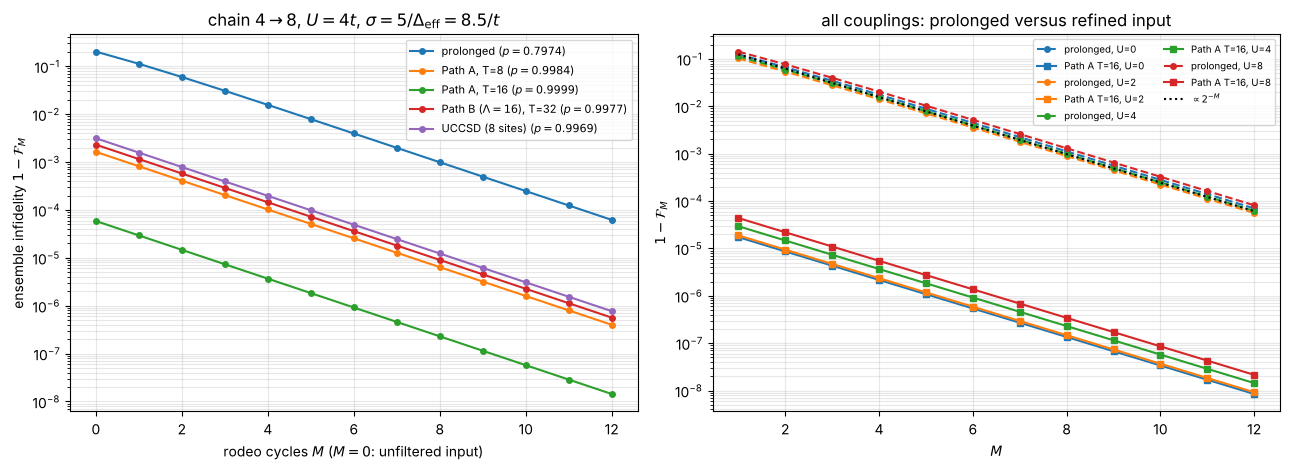
\includegraphics[width=\textwidth]{figs/fig6.png}
  \caption{Exact ensemble infidelity of the rodeo filter,
  Eq.~\eqref{eq:fid}, with $\sigma=5/\Deff$ versus the number of cycles.
  Left, $U=4t$: prolonged input, Path-A inputs refined for $T=8/t$ and
  $16/t$, the Path-B input at its ceiling and the eight-site UCCSD state.
  Right: prolonged (dashed) and Path-A $T=16/t$ (solid) inputs for all four
  couplings against the $2^{-M}$ law.}
  \label{fig:rodeo}
\end{figure*}

% ===========================================================================
\section{Ingredients of the thirty-two-qubit study}
\label{sm:large}
% ===========================================================================
\paragraph{Product formulas through the Kronecker structure.}
In the $(2,2)$ sector of the sixteen-site chain ($14\,400$ states) the dense
machinery of the eight-site study is unavailable: a $14\,400^2$ complex step
unitary cannot be stored, let alone diagonalized.  Every term of the
product formula is instead applied through Eq.~\eqref{eq:kron}.  A hopping
layer $K_{\rm layer}=K_\uparrow\otimes\mathbb1+\mathbb1\otimes K_\downarrow$
acts on $\psi$ reshaped as a $120\times120$ matrix as
$e^{-icK_\uparrow}\,\Psi\,e^{-icK_\downarrow^T}$, with the two $120\times120$
exponentials obtained from one diagonalization per species; the diagonal
interaction is an elementwise phase; and the embedded coarse term of Path~A,
$P\,X\,P^\dagger$ with $X$ one of the three $784\times784$ conditioned coarse
groups, is applied exactly as
$\psi\mapsto\psi+P\big[V(e^{-ic\lambda}-1)V^\dagger\big]P^\dagger\psi$, with
$X=V\lambda V^\dagger$ diagonalized once.  The second-order step is the
symmetric product of these factors.  The ramp uses the groups
$[K_{\rm even},K_{\rm odd},D]$ with the interaction coefficient
$\sin^2(\pi s/2)$, Path~B the same groups with the even (intra-block) layer
scaled by $1+\Lambda\cos^2(\pi s/2)$, and Path~A the six groups
$[P(D_c-\mu)P^\dagger,PK^c_{\rm even}P^\dagger,PK^c_{\rm odd}P^\dagger,
K_{\rm even},K_{\rm odd},D-\mu]$ with the $\cos^2$/$\sin^2$ coefficients of
Eq.~\eqref{eq:pathA}.  The exact-slice transports use $48$ slices with a
sparse Krylov exponential.  Applied to the eight-site chain, where the
dense machinery exists, the Kronecker implementation reproduces the ramp,
the split-group Path-A refinement and the filter tracks of
Sec.~\ref{sec:budget} to $10^{-13}$.

\paragraph{The Trotter-effective ground state.}
The fixed-step filter projects, in the long run, on the eigenvector of the
step unitary $U_{\delta t}$ closest to the ground state, and its eigenphase
is the objective energy $\Eobj$.  At eight sites that eigenvector was read
off a Schur decomposition of the step; at sixteen sites it is obtained by
iterating the quantized-time filter itself: starting from the exact ground
state, $\psi\mapsto\tfrac12(\psi+e^{i\Eobj n\delta t}U_{\delta t}^n\psi)$
with $n$ drawn from the Gaussian ensemble of cycle times and $\Eobj$
updated at every iteration to the eigenphase estimate
$-\arg\expval{U_{\delta t}}{\psi}/\delta t$, converges in a few tens of iterations to the fixed point of the
filter, which is that eigenvector.  At eight sites the procedure reproduces
the Schur result ($\Eobj=-5.620907$, floor $5.8\times10^{-5}$) to the
quoted digits; at sixteen sites, with $\sigma=36.2/t$ and $\delta t=0.1/t$,
it gives $\Eobj-E_0=+4.92\times10^{-3}t$ and a floor of
$3.7\times10^{-5}$, close to the eight-site floor at the same step, as
expected for a local error per step that is the same at both sizes.

\paragraph{Gate counts at sixteen sites.}
The second-order step of the sixteen-site chain costs $304$ CNOTs ($736$
controlled), the Givens network of the free-fermion determinant
$2\times120$ rotations, $480$ CNOTs, the prolongation $8\to16$ $32$ CNOTs,
and the coarse term of Path~A --- the eight-site Hubbard step, $48$
rotations, conditioned on the sixteen antibonding qubits with the
relative-phase Toffoli ladder --- $4\,856$ CNOTs per application, applied
twice per second-order step.  The preparation of the coarse eigenstate
itself is counted, for every input that starts from it, at the cost of the
cheapest eight-site route of Table~\ref{tab:budget} that reaches
$3\times10^{-4}$, the ramp at $T=16/t$ without filtering ($18\,544$ CNOTs);
its residual infidelity ($3.4\times10^{-4}$) is below the targets of the
sixteen-site comparison and is neglected.

\paragraph{Step scans.}
With the step scans of the notebook (second order, $n_s=32$ to $512$,
accepted when the overlap agrees with the exact-slice value to $10^{-3}$ or
has stopped changing): the ramp needs $n_s=128$ at $T=16/t$ ($0.96927$
against $0.96970$; $0.91802$ at $n_s=64$) and $256$ at $T=32/t$ ($0.99556$
against $0.99591$; $0.00545$, $0.94463$ and $0.99304$ at $n_s=32$, $64$,
$128$ --- a step of $\delta t=1/t$ destroys the transport); Path~B with
$\Lambda=8t$ needs $256$ at $T=16/t$ ($0.99476$ against $0.99492$;
$4\times10^{-5}$, $0.266$ and $0.98688$ at $n_s=32$, $64$, $128$, the
intra-block generator of norm $1+\Lambda$ requiring $\delta t\lesssim0.06/t$),
and is not Trotterized at $T=32/t$, where it sits at the same ceiling and
would need $512$ steps; Path~A with $\mu_{\rm buf}=2t$ and the
coarse groups split needs $n_s=128$ at $T=16/t$ ($0.99835$ against
$0.99931$) while at $T=8/t$ it plateaus at $0.99079$ from $n_s=128$ on
($0.98885$, $0.99069$, $0.99078$, $0.99079$, $0.99079$ at
$n_s=32$--$512$) against the exact $0.99237$, a residual of
$1.6\times10^{-3}$ that no step count removes --- the product formula with
the coarse term split into non-commuting groups follows a slightly different
path, whose end point differs from the exact one by more than the tolerance
when the transport is this short.

\paragraph{Sector gap along the ramp.}
The sector gap of $H_R(s)$ falls monotonically from $0.165t$ at $s=0$ to
$0.051t$ at $s=1$ ($0.125t$, $0.078t$, $0.057t$ at $s=0.25,0.5,0.75$); the
ramp from the determinant is governed, like Path~A, by the gap in the
singlet, reflection-even sector, which is why both transports converge at
all with a sector gap of $0.05t$.

% ===========================================================================
\section{Operating points}
\label{sm:ops}
% ===========================================================================
Table~\ref{tab:ops} gives, for the eight-site comparison of
Table~\ref{tab:budget}, the minimum CNOTs per accepted preparation with
which each input reaches a target ensemble infidelity, with the number of
cycles that attains it; the corresponding operating points at sixteen sites
are the last four columns of Table~\ref{tab:large}, read from the twenty
time sets with relative standard errors of $10$--$35\%$ at the cycle counts
involved; Table~\ref{tab:largefull} gives the sixteen-site data in full.

\begin{table*}[t]
  \caption{Operating points at eight sites: the minimum CNOTs per accepted
  preparation with which each input of Table~\ref{tab:budget} reaches a
  target ensemble infidelity, with the number of cycles $M$ that attains it
  in parentheses ($M\le6$; a dash means the target is not reached within
  six cycles).}
  \label{tab:ops}
  \centering\scriptsize
  \begin{tabular}{lccc}
  \toprule
  input & $10^{-3}$ & $3{\times}10^{-4}$ & $10^{-4}$\\
  \midrule
  prolonged / determinant & --- & --- & ---\\
  UCCSD pruned & $6.2{\times}10^{4}$ (2) & $1.2{\times}10^{5}$ (4) & ---\\
  UCCSD full & $7.8{\times}10^{4}$ (2) & $1.3{\times}10^{5}$ (4) & ---\\
  ramp, $T=8$ & $5.6{\times}10^{4}$ (2) & $1.1{\times}10^{5}$ (4) & $1.5{\times}10^{5}$ (6)\\
  ramp, $T=16$ & $1.9{\times}10^{4}$ (0) & $4.0{\times}10^{4}$ (1) & $9.1{\times}10^{4}$ (3)\\
  Path B, $\Lambda=8t$ & $1.4{\times}10^{5}$ (4) & $1.6{\times}10^{5}$ (5) & ---\\
  Path A & $3.0{\times}10^{5}$ (0) & $3.0{\times}10^{5}$ (0) & $3.4{\times}10^{5}$ (2)\\
  \bottomrule
  \end{tabular}
\end{table*}


\begin{table*}[t]
  \caption{The sixteen-site matched comparison of Table~\ref{tab:large} in
  full: ensemble infidelity (bootstrap relative standard error in
  parentheses) and CNOTs per accepted preparation after $M=0$, $2$, $4$ and
  $6$ cycles, and the cumulative acceptance after six.}
  \label{tab:largefull}
  \centering\scriptsize
  \setlength{\tabcolsep}{3pt}
  \resizebox{\textwidth}{!}{\begin{tabular}{lc|cc|cc|cc|ccc}
  \toprule
  input & $p$ & \multicolumn{2}{c|}{$M=0$} & \multicolumn{2}{c|}{$M=2$} & \multicolumn{2}{c|}{$M=4$} & \multicolumn{3}{c}{$M=6$}\\
  & & $1-\mathcal F$ & CNOTs & $1-\mathcal F$ & CNOTs & $1-\mathcal F$ & CNOTs & $1-\mathcal F$ & CNOTs & $P_6$\\
  \midrule
  determinant & 0.7162 & $2.8{\times}10^{-1}$ & 480 & $8.9{\times}10^{-2}$ (6\%) & $5.5{\times}10^{5}$ & $2.7{\times}10^{-2}$ (10\%) & $1.1{\times}10^{6}$ & $7.1{\times}10^{-3}$ (18\%) & $1.5{\times}10^{6}$ & 0.717\\
  prolonged & 0.8692 & $1.3{\times}10^{-1}$ & 18\,576 & $3.9{\times}10^{-2}$ (6\%) & $5.2{\times}10^{5}$ & $1.1{\times}10^{-2}$ (16\%) & $1.0{\times}10^{6}$ & $2.4{\times}10^{-3}$ (13\%) & $1.4{\times}10^{6}$ & 0.870\\
  UCCSD pruned (255) & 0.9930 & $7.0{\times}10^{-3}$ & 87\,776 & $1.9{\times}10^{-3}$ (10\%) & $5.6{\times}10^{5}$ & $5.6{\times}10^{-4}$ (15\%) & $1.1{\times}10^{6}$ & $1.3{\times}10^{-4}$ (12\%) & $1.5{\times}10^{6}$ & 0.993\\
  ADAPT (187 op.) & 0.9901 & $9.9{\times}10^{-3}$ & 68\,008 & $2.6{\times}10^{-3}$ (8\%) & $5.4{\times}10^{5}$ & $7.2{\times}10^{-4}$ (14\%) & $1.0{\times}10^{6}$ & $1.7{\times}10^{-4}$ (11\%) & $1.4{\times}10^{6}$ & 0.990\\
  ramp, $T=16$, $n_s=128$ & 0.9693 & $3.1{\times}10^{-2}$ & 39\,392 & $7.7{\times}10^{-3}$ (17\%) & $5.2{\times}10^{5}$ & $2.0{\times}10^{-3}$ (19\%) & $1.0{\times}10^{6}$ & $4.2{\times}10^{-4}$ (35\%) & $1.4{\times}10^{6}$ & 0.970\\
  ramp, $T=32$, $n_s=256$ & 0.9956 & $4.4{\times}10^{-3}$ & 78\,304 & $1.1{\times}10^{-3}$ (21\%) & $5.5{\times}10^{5}$ & $3.2{\times}10^{-4}$ (20\%) & $1.0{\times}10^{6}$ & $8.6{\times}10^{-5}$ (23\%) & $1.4{\times}10^{6}$ & 0.996\\
  Path B ($\Lambda=8t$), $T=16$, $n_s=256$ & 0.9948 & $5.2{\times}10^{-3}$ & 96\,400 & $1.4{\times}10^{-3}$ (7\%) & $5.7{\times}10^{5}$ & $4.3{\times}10^{-4}$ (13\%) & $1.1{\times}10^{6}$ & $1.4{\times}10^{-4}$ (13\%) & $1.5{\times}10^{6}$ & 0.995\\
  Path A (split), $T=16$, $n_s=128$ & 0.9983 & $1.7{\times}10^{-3}$ & 1\,300\,624 & $4.3{\times}10^{-4}$ (17\%) & $1.8{\times}10^{6}$ & $1.7{\times}10^{-4}$ (25\%) & $2.3{\times}10^{6}$ & $7.4{\times}10^{-5}$ (17\%) & $2.7{\times}10^{6}$ & 0.998\\
  \bottomrule
  \end{tabular}}
\end{table*}

\begin{thebibliography}{9}
\bibitem{Jansen2007} S.~Jansen, M.-B.~Ruskai, and R.~Seiler, J.~Math.\ Phys.\
\textbf{48}, 102111 (2007).
\end{thebibliography}

\end{document}
